\subsection{Design of the dataflow}\label{subsec:dataflow}

\textbf{work in progress}

Gathering and structuring the data in this project is quite a challenge. The stores and retailers do not publish official prices of all their products, they only issue a catalog items on sale. These items on sale, or offers, are published in a new catalog each week. The figure \figref{fig:dataflow} shows the complete design of the dataflow for our solution. It illustrates the complexity of gathering information from different sources and presenting them to the user. Recipes have to be gathered from a free website or from the users using the application. But we need some sort of storage for recipes, to enable people to actually use the application in the first place. When we are able to store recipes, we need to fill our database with actual recipes from somewhere. Opskrifter.dk is a huge online database with around 3.000 different recipes, and these are the recipes we intend to use and work with in our application. This part may seem rather trivial, however adjusting recipes for spelling errors and matching them with the right ingredients can be problem. This error checking and matching requires some string analysis and word management. It will be possible for us as the developers to control and maintain the data, and additionally a lot of the work have to be done manually, because it is extremely challenging to catch all of the problems with the recipes.

In this project we need a strong foundation of ingredient data. We want to match both recipes and offers to specific types of ingredients. This will allow us to compute the cost of buying certain ingredients for a recipe, including ingredients on sale, which we decided to call offers. Ingredient data is more complicated because no complete list exists. We bought a data-sheet from Statistics Denmark which contains the average prices of groceries, across stores and retailers. Groceries can be ingredients or food items used to cook. We want to use these as a base for all calculations we do. All of this data is functioning as a good base, it does however not portray a completely true image of each store and retailer. It will resolve in some values as to what you save and actual price, that wont be 100\% correct -which is why our application may only can be seen as a guidance and estimate of the price and savings, not guaranteeing to be the exact price. The offers for the different groceries are gathered through \textit{eTilbudsAvisen}. It is an online service which gathers all offers offered by a selection of retailers in Denmark, and it does so by traversing the catalogs and extracting all the data. They offer all their data through a web based application programming interface (API), and the idea is that we will download the relevant data from their database once a day, and make the calculations necessary for it to match our database. 

\begin{figure}
\label{fig:dataflow}
\centering
\includegraphics[width=0.95\textwidth]{Pictures/dataflow}
\caption{A model of the dataflow through the entire system}
\end{figure}

\paragraph{Design of the Database}
\label{para:dbdesign}

Data is a big part of this project. Data is content, data is what makes the users want to start, and continue using the application. Obviously, we want to handle the data in a uniform and structured way, which is the reason why we designed and implemented a database. A big part of the application is dependent upon the database being frequently and correctly updated. Furthermore the database has to be designed in a way that makes calculations fast to compute and access, as we do not want the user to wait for long queries and joins in order to get something shown on the application. We will have huge amount of data, with a daily update requirement and further backend development.



\begin{figure}
\label{fig:ER-diagram}
\centering
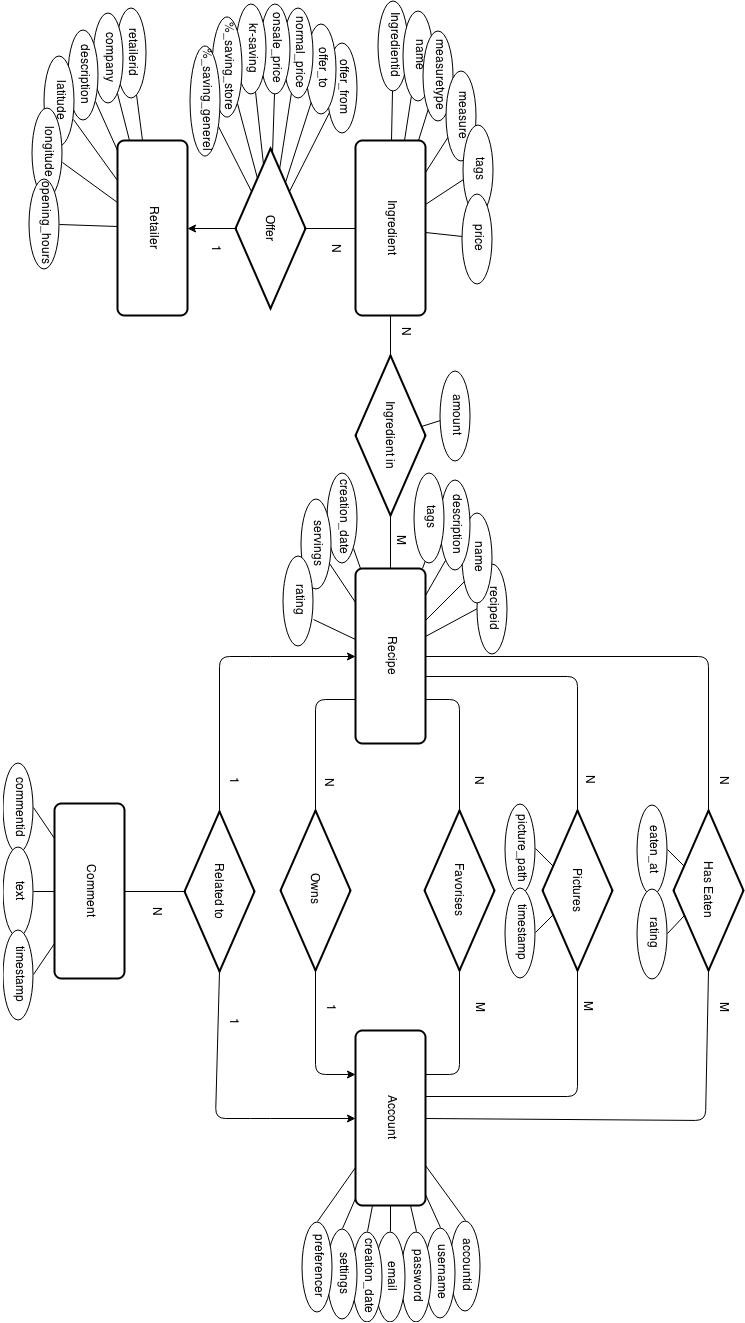
\includegraphics[width=0.95\textwidth]{Pictures/ERdiagram}
\caption{The final ER diagram of the database}
\end{figure}

A lot of these relations speak for themselves, and the entire amount of relationships between account and recipe rather intuitive. We have chosen not to gather all the data in a single relationship as we want perform quick queries on the database rather than save memory. This is one of the advantages of having a stationary server with a large amount of memory available, it is possible to focus solely on performance. 

The biggest table in terms of sheer numbers would be ingredientIn, as each recipe has a lot of different ingredients. This has been accommodated for by moving most attributes to either recipe or ingredient, and we make sure to query through IngredientIn before joining any of these together.

